\subsection{Socials}

\subsubsection{Illini Union Rec Room Lockout}
The Illini Union Rec Room is located in the basement of the Union building. A Rec Room lockout gives ANS exclusive access to 14 bowling lanes, 12 billiard tables, and coin-operated arcade games following dinner at the Krannert Center for Performing Arts, only a short walk away through the University of Illinois main quad! This space can accompany up to 150 people, with extra tables outside of the Rec Room for socializing, playing board games, or having a late night snack or coffee with professionals or students from other universities.
\vspace{0.5cm}\newline
% Illini Union Rec Room Picture
\begin{figure}[H]
	\centering
	\begin{subfigure}{0.5\textwidth}
		\centering
		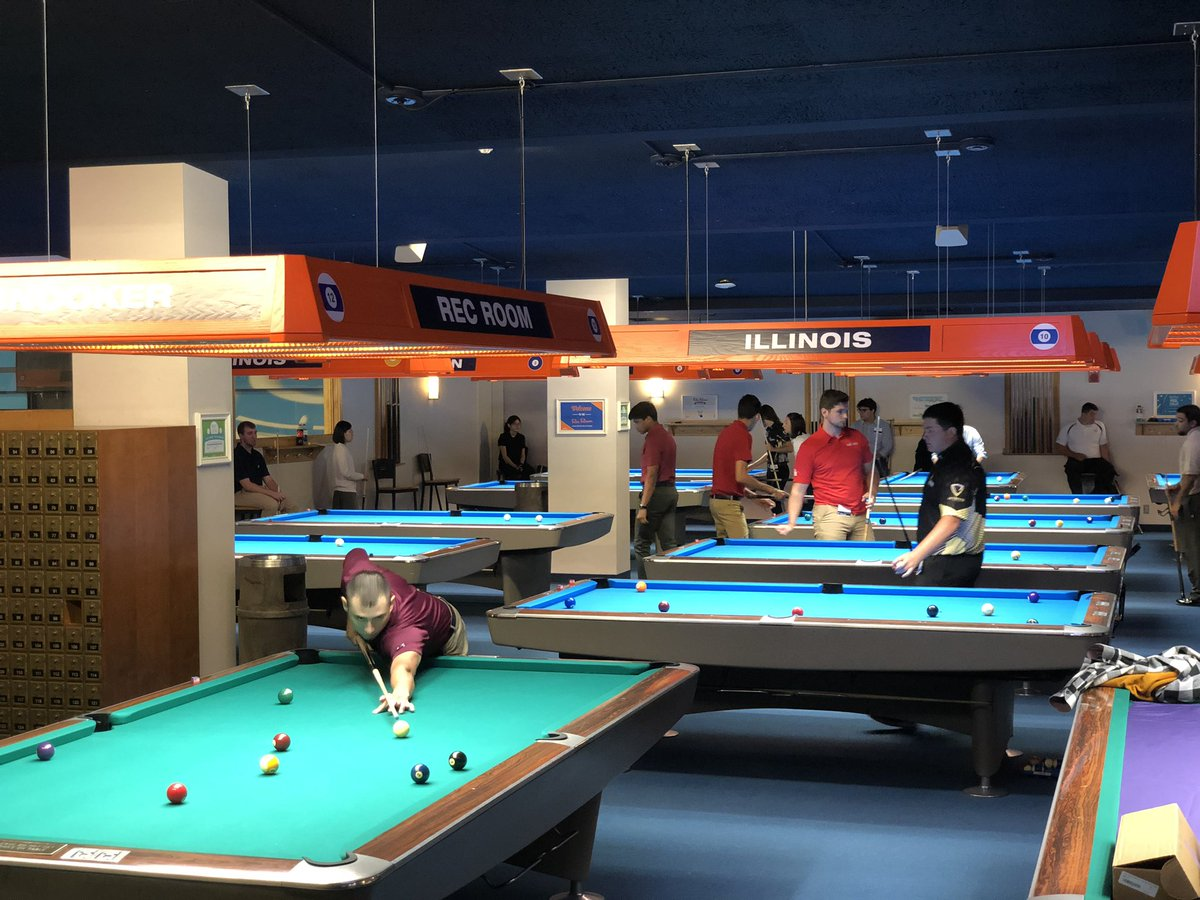
\includegraphics[width=0.9\linewidth]{union_recroom1.png}
	\end{subfigure}%
	\begin{subfigure}{0.5\textwidth}
		\centering
		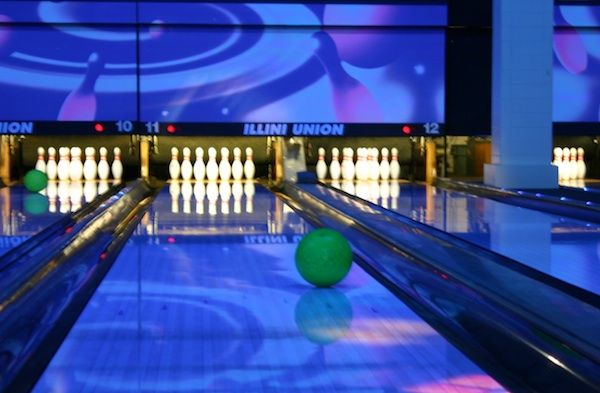
\includegraphics[width=0.9\linewidth]{union_recroom2.png}
	\end{subfigure}	
	\caption{Illini Union Rec Room}	
\end{figure} 

\subsubsection{77 Club at Memorial Stadium}
Memorial Stadium is not only home to the Fighting Illini football team, but also to exquisite event space overlooking Zuppke Field. The sixth level of Memorial Stadium is home of the magnificent 77 Club, which honors Illini great, the ``Galloping Ghost'' Red Grange. This 5,020 square foot space is located midfield and features an outdoor patio area overlooking the city of Champaign, for a combined total space of 9,740 square feet. This event will take place following dinner at I Hotel Conference Center, and is just a short and scenic walk away past the State Farm Center (formerly the historic Assembly Hall). Tables will be set up around a stage featuring live music and a dance floor and drinks will be served. This is the perfect event to incorporate a little bit of Illinois history with music, dancing, and socializing! 
\vspace{0.5cm}\newline
% 77 Club Picture
\begin{figure}[H]

	\centering
	\begin{subfigure}{0.5\textwidth}
		\centering
		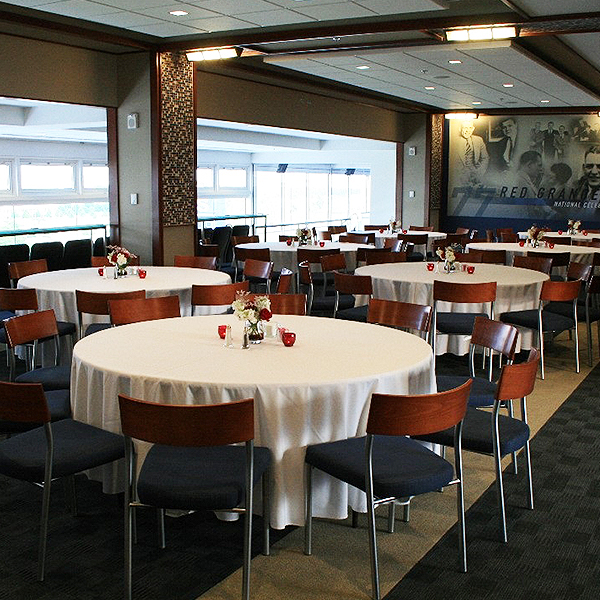
\includegraphics[width=0.7\linewidth]{77club1.png}
	\end{subfigure}%
	\begin{subfigure}{0.5\textwidth}
		\centering
		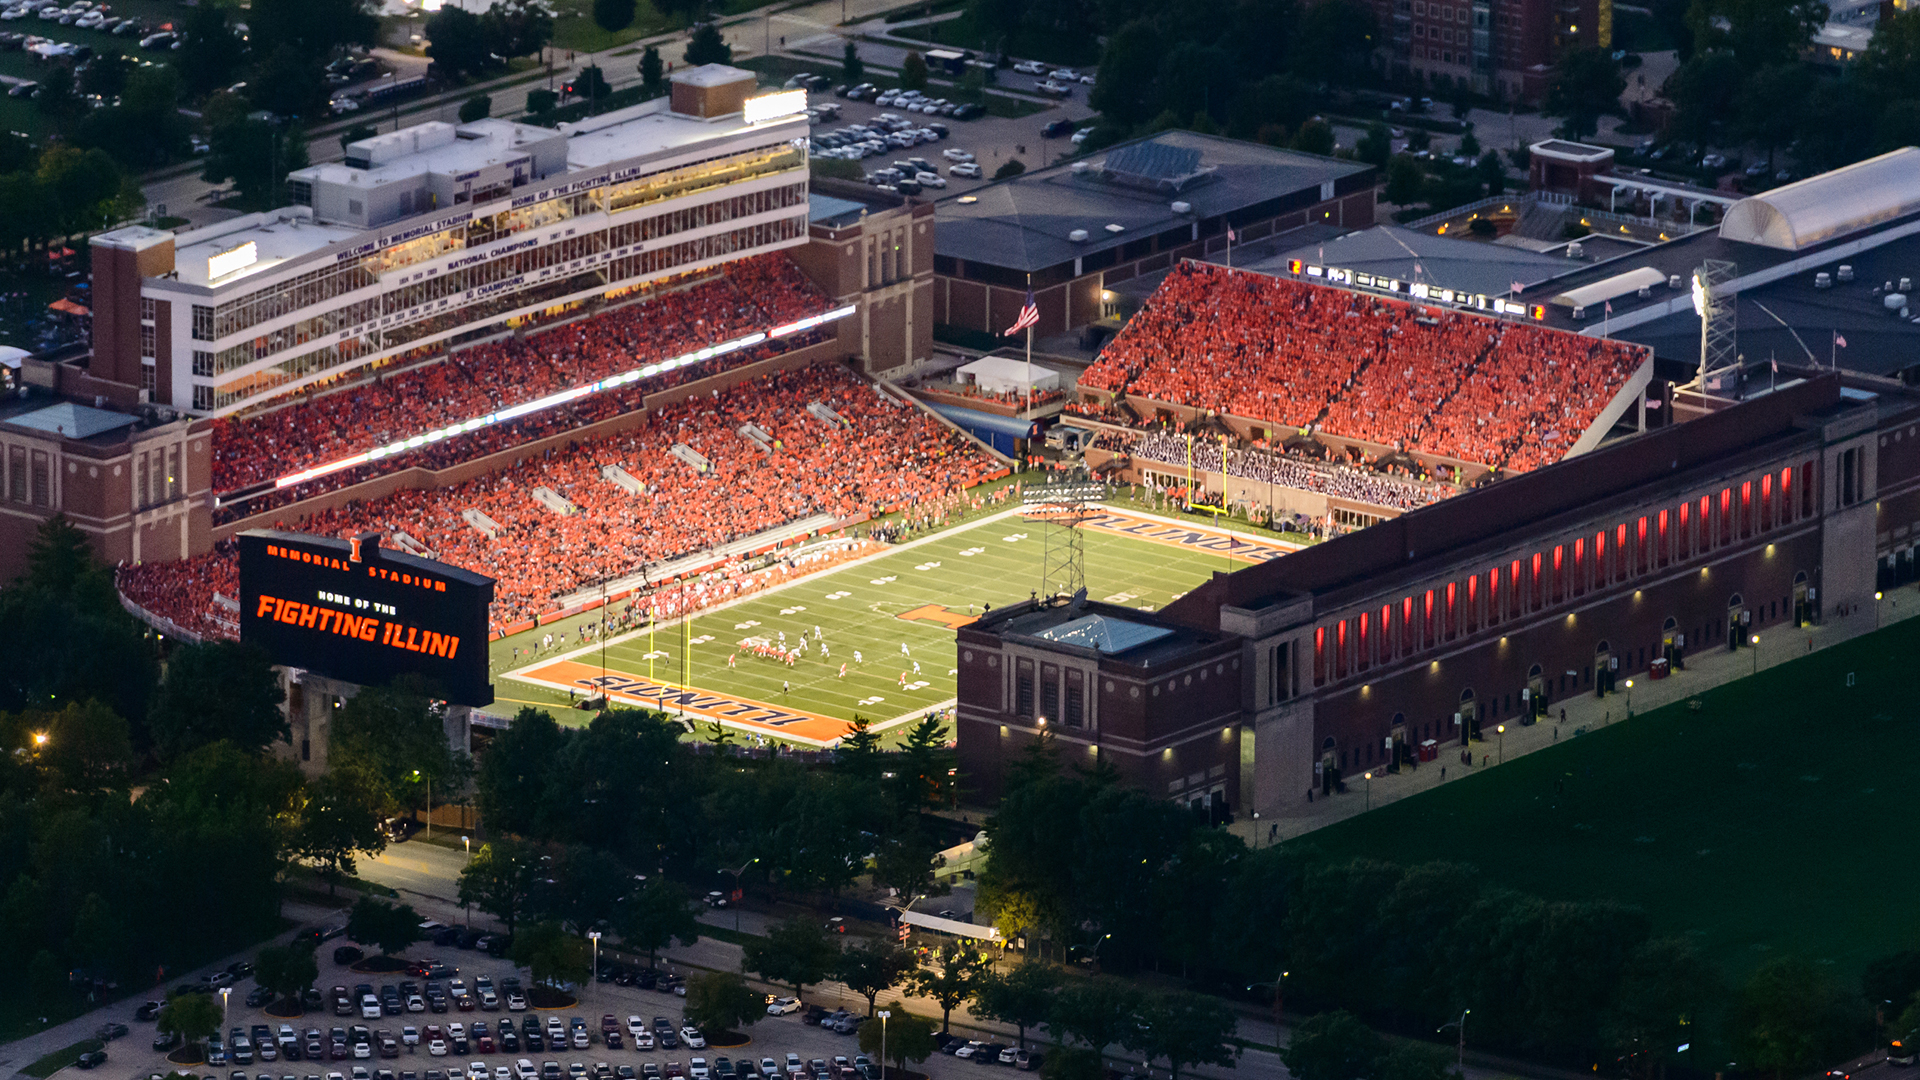
\includegraphics[width=0.9\linewidth]{77club2.png}
	\end{subfigure}
	\caption{77 Club at Memorial Stadium}		
\end{figure} 

%%% Reserve for Pour Bros. social %%%
%\subsubsection{Pour Bros. Taproom in Downtown Champaign}
%Welcome to Illinois' first pour-your-own taprooms. Pour Bros. Taproom is located in the heart of the historic downtown Champaign area and features 28 pour-your-own taps: beers, ciders, meads and wine\ldots all poured by you, one ounce at a time. Socialize over the vintage games Pour Bros has to offer: skeeball, bubble hockey, steel tip darts, DAGZ and more! If you are feeling more on the leisurely side, Pour Bros features live music in a spacious and comfortable seating area for you to get your networking on.
%\vspace{0.5cm}\newline
%% Pour Bros Picture
%\begin{figure}[H]
%
%	\centering
%	\begin{subfigure}{0.5\textwidth}
%		\centering
%		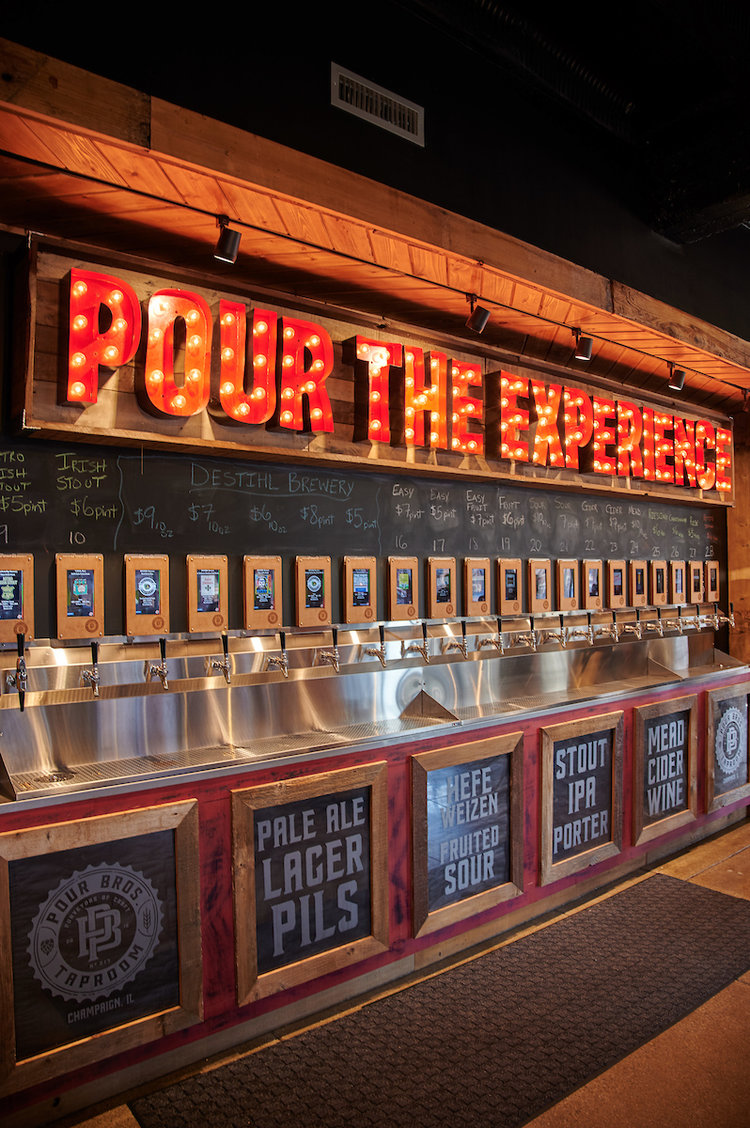
\includegraphics[width=0.5\linewidth]{pour_bros2.png}
%	\end{subfigure}%
%	\begin{subfigure}{0.5\textwidth}
%		\centering
%		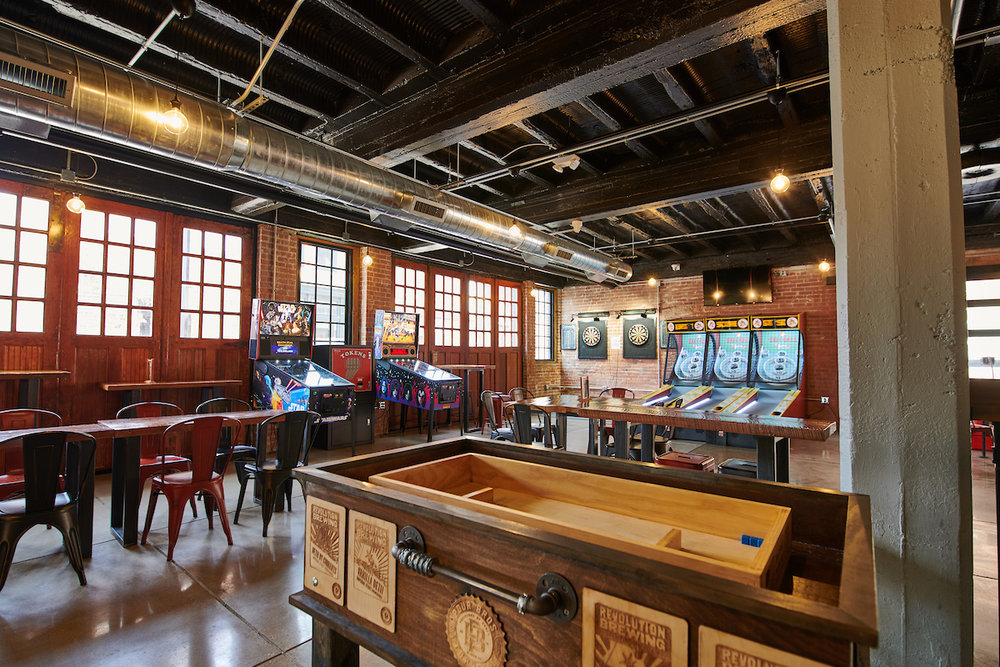
\includegraphics[width=0.9\linewidth]{pour_bros1.png}
%	\end{subfigure}	
%	\caption{Pour Brothers Taproom}	
%\end{figure} 

\subsubsection{Barn Dance: A Proud Midwestern Tradition}
Barn dances are a staple event at UIUC. Socialize in a unique environment with games of corn-hole and other midwestern fun. Various barns are used for dancing and mingling by many of the student organizations on UIUC campus, such as Farm Lake barn which hosts dozens of barn dances annually. Other barns may be best suited for the student conference social events, such as Hudson Farm, which offers a corporate event or professional social events option which can accommodate up to 300 guests with an alcohol service available and friendly, helpful service. Like socials in the past student conferences, the barn may be used and a third party service can be hired to bring the square dance, swing dance, two step and cowboy boogie to the barn dance floor! 
\vspace{0.5cm}\newline
% Barn Dance Hudson Picture
\begin{figure}[H]
	\centering
	\begin{subfigure}{0.4\textwidth}
		\centering
		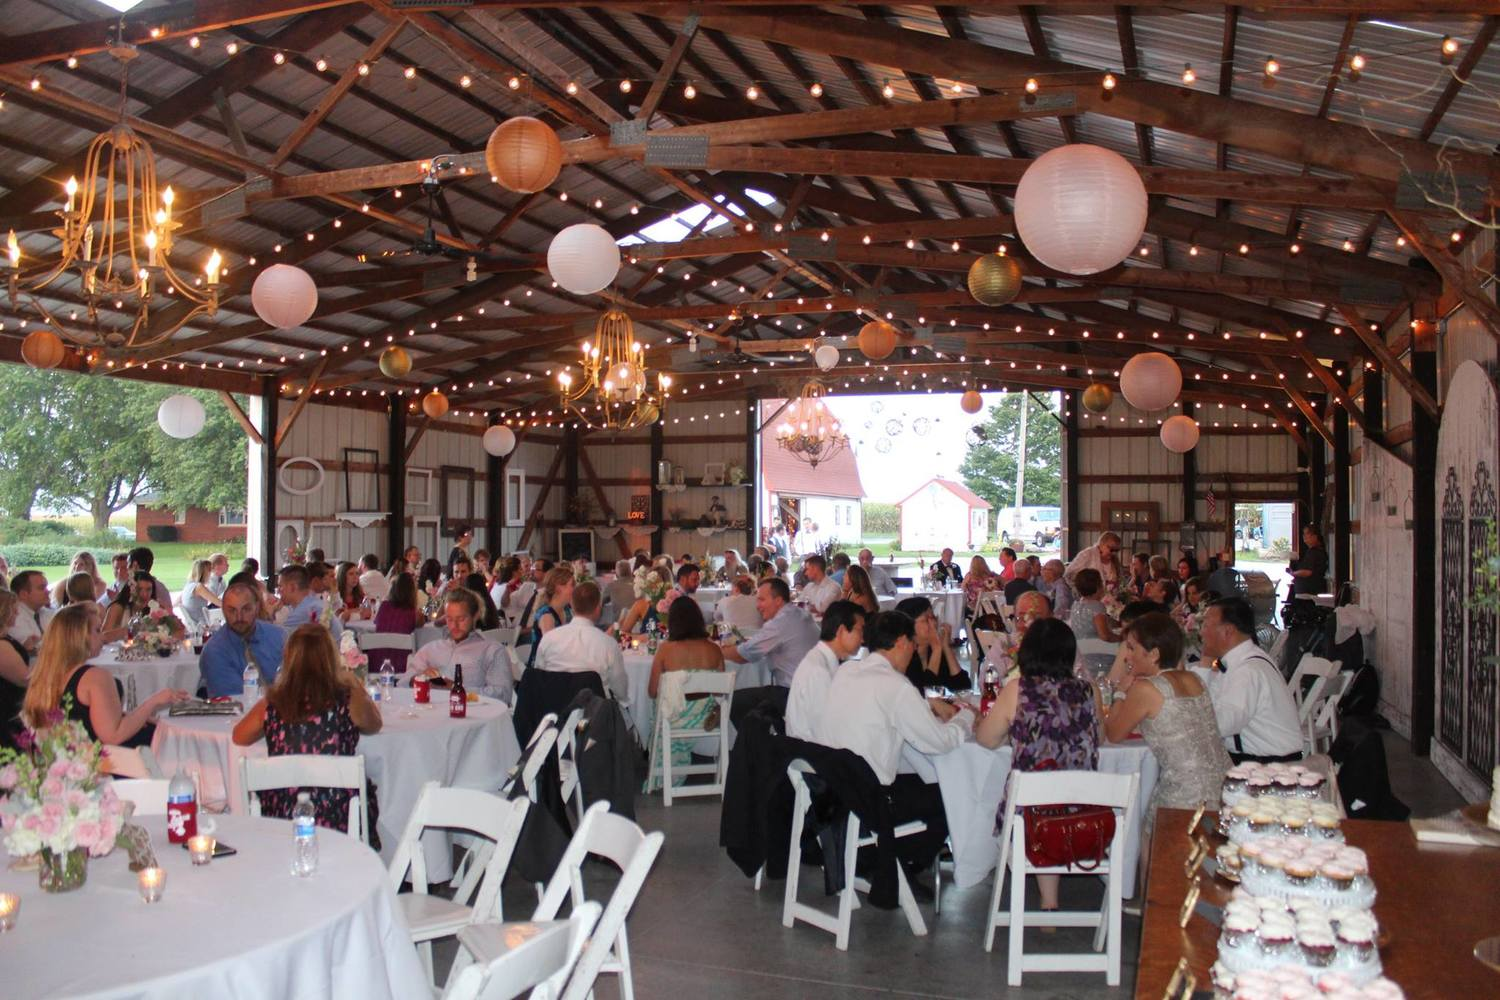
\includegraphics[width=0.9\linewidth]{barn_dance1.png}
	\end{subfigure}%
	\begin{subfigure}{0.4\textwidth}
		\centering
		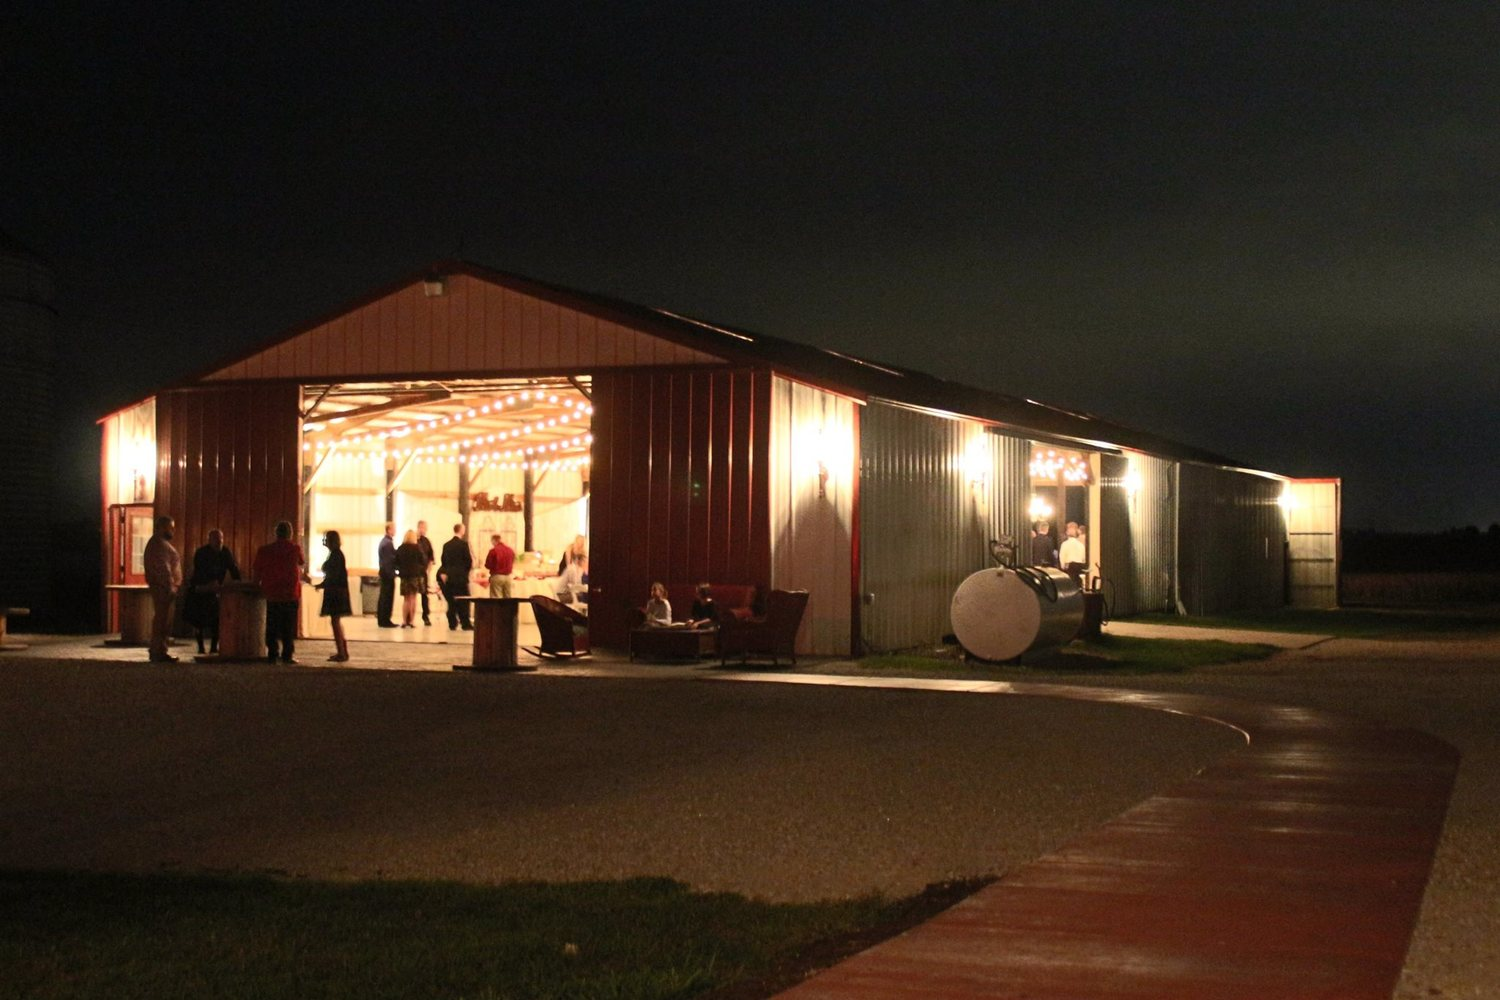
\includegraphics[width=0.9\linewidth]{barn_dance2.png}
	\end{subfigure}	
	\caption{Hudson Farm Barn.}	
\end{figure} 
\begin{figure}[H]
	\centering
	\begin{subfigure}{0.4\textwidth}
		\centering
		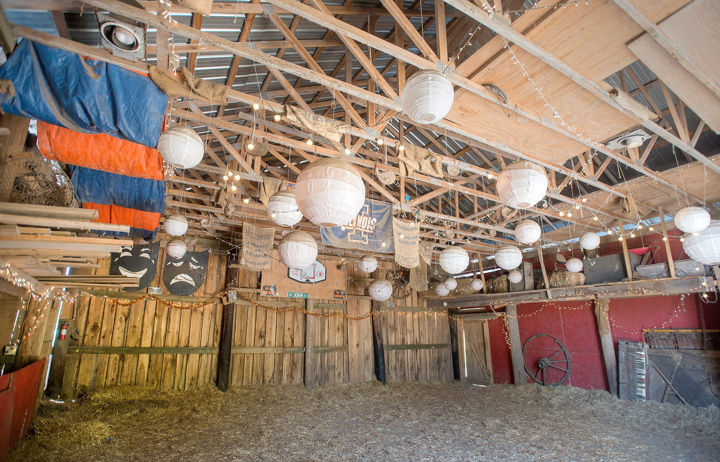
\includegraphics[width=0.9\linewidth]{farmlake1.jpg}
	\end{subfigure}%
	\begin{subfigure}{0.4\textwidth}
		\centering
		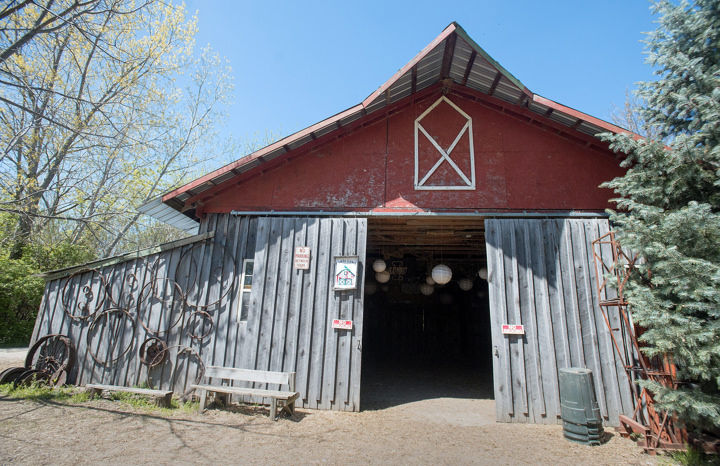
\includegraphics[width=0.9\linewidth]{farmlake2.jpg}
	\end{subfigure}	
	\caption{Farm Lake Barn}	
\end{figure} 

\subsubsection{Under 21 Social: University of Illinois Ice Arena}
For students under the drinking age that cannot attend the Pour Bros. Taproom social event, the University of Illinois Ice Arena is another option that is only a brief walking distance from the Union. It was built in 1931 and offers a unique option for skating get-togethers from broomball and hockey to group skating parties. The Ice Arena is a 55,000 square foot facility and is the only one in Champaign-Urbana. The dimensions of the rink are 192' by 115' with a 1,200 seat arena surrounding. There are four public locker rooms, four party areas, and two Zambonis in the facility. The Center Ice Cafe offers hot chocolate, coffee, smoothies, fountain drinks, and more to quench your thirst.  Snacks and concession items are also available.
\vspace{0.5cm}\newline
% Ice Arena Picture
\begin{figure}[H]
	\centering
	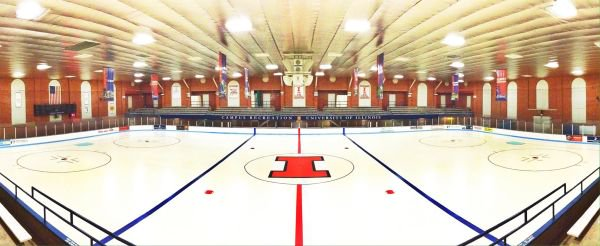
\includegraphics[width=0.8\textwidth]{ice_arena.png}
	\caption{The UIUC Ice Arena}
\end{figure}

